\documentclass[a4paper,twoside,11pt]{report}
\usepackage[italian]{babel}
\usepackage[utf8x]{inputenc}
%\usepackage[latin1]{inputenc}
\usepackage[T1]{fontenc}
%\usepackage[scaled]{helvet}
%\renewcommand\familydefault{\sfdefault}

%\renewcommand{\sfdefault}{cmr}
%helvetica
%\renewcommand{\sfdefault}{phv}
%courier
%\renewcommand{\sfdefault}{pcr}
\usepackage{listings}
\usepackage{color}
\usepackage{caption}
\usepackage{subcaption}
\usepackage{sidecap}
\usepackage{quoting}
\quotingsetup{font=small}
\usepackage{eurosym}
\usepackage{graphicx}
\usepackage{epsfig}
\usepackage{url}
\usepackage{comment}
\usepackage{amsmath}
\usepackage[dvipsnames]{xcolor}
%%https://en.wikibooks.org/wiki/LaTeX/Colors
\usepackage[colorlinks]{hyperref}
%\hypersetup{hidelinks}

\hypersetup{%
	,urlcolor=Cyan
	,citecolor=black
	,linkcolor=black
}

\lstdefinestyle{customc}{
	belowcaptionskip=1\baselineskip,
	breaklines=true,
	frame=L,
	%xleftmargin=\parindent,
	language=C++,
	showstringspaces=false,
	basicstyle=\footnotesize\ttfamily,
	keywordstyle=\bfseries\color{green!40!black},
	commentstyle=\itshape\color{purple!40!black},
	identifierstyle=\color{blue},
	stringstyle=\color{orange},
}

\lstdefinestyle{customasm}{
	belowcaptionskip=1\baselineskip,
	frame=L,
	%xleftmargin=\parindent,
	language=[x86masm]Assembler,
	basicstyle=\footnotesize\ttfamily,
	commentstyle=\itshape\color{purple!40!black},
}

\lstset{escapechar=@,style=customc}


%opening
\title{Programmazione di Sistemi Embedded\\ {\Large Jimmy Challenge Arduino Game}}
\author{
    Edoardo Rosa - Matr. 707922\\
    Federico Torsello - Matr. 702619}

                             % \ip that is commented out.

\begin{document}             % End of preamble and beginning of text.
\maketitle                   % Produces the title.
\begin{abstract}

In questa relazione si descriverà come è stato progettato il gioco interattivo \textbf{Jimmy Challenge}, descrivendo le scelte di progettuali e le fasi implementative.

Jimmy Challenge è stato realizzato utilizzando diversi componenti hardware/software, con l'obiettivo di sfruttare ed ottimizzare quanto più possibile la board Arduino in un'ottica IoT.

\begin{description}
	\item [Capitolo 1] In questo capitolo si introduce il progetto e l'interazione giocatore-sistema.
	\item [Capotolo 2]
	
	
\end{description}


\end{abstract}
 %Sommario
\chapter{Introduzione}
\textbf{Jimmy Challenge}\footnote{"\textit{jimmy}" in inglese vuol dire grimaldello, da questo il nome del gioco.} è un gioco interattivo che si ispira all'attività di \textit{lock-picking}: aprire un lucchetto o una serratura usando ad esempio un \textbf{grimaldello} per manipolare i pistoncini interni per simulare la presenza della chiave originale.

Per poter giocare è necessario alimentare l'\href{https://www.arduino.cc/en/Main/ArduinoBoardUno}{Arduino UNO\footnote{Arduino UNO - è una scheda elettronica di piccole dimensioni con un microcontrollore ATmega, utile per creare rapidamente prototipi e per scopi hobbistici, didattici e professionali. (\url{https://it.wikipedia.org/wiki/Arduino\_\%28hardware\%29})}} e attendere qualche secondo di setup.

Una volta che il settaggio è completo, l'utente può interagire con Arduino utilizzando diversi componenti hardware che mutano il loro comportamento in base al contesto.





\chapter{Progettazione di un sistema Embedded}
\section{Analisi dei requisiti}
\subsection{Requisiti funzionali}
Il sistema realizzato deve permettere ad uno o due giocatori di competere per sbloccare dei lucchetti. Ad ogni lucchetto sbloccato si supera il livello fino a quando i livelli non terminano e il gioco si dice finito. Durante il gioco sono presenti delle penalità e dei bonus.

\subsection{Requisiti non funzionali}
Le performance utili per la buona riuscita del progetto a cui non si può rinunciare riguardano la rilevazione della distanza e l'invio dei feedback locali/remoti.
Il tempo gioca un ruolo importante in questo progetto, quindi si devono evitare inutili ritardi nella rilevazione ed invio delle informazioni.

\section{Modeling}
Il sistema si suddivide in più parti:
\begin{itemize}
	\item parte fisica lato client/server
	\item parte software lato client/server
	\item networking lato client/server
\end{itemize}

\subsection{Modellazione della parte fisica - lato client}
Dal punto di vista fisico, si ha un Arduino UNO:
 \begin{itemize}
 	\item connesso ad una breadboard e a dei componenti hardware attraverso i sui pin digitali
 	\item connesso ad un PC mediante la porta USB (da cui riceve l'alimentazione a 5v). 
 \end{itemize}
 Ogni componente della breadboard ha un proprio impiego distinguendoli in \textbf{sensori} ed \textbf{attuatori} secondo la visione di \textit{sistema reattivo}.

	\begin{quote}
		\textbf{Reactive system}: è l’ambiente esterno che determina gli eventi che
		condizionano l’esecuzione del sistema
	\end{quote}
	
La connessione seriale via USB serve per inviare i dati campionati dall'Arduino verso il PC. A loro volta questi dati possono servire per creare una GUI locale (per esempio su terminale) o remota, su browser.

\subsection{Modellazione della parte logica - lato client}
Per realizzare il comportamento dinamico del progettare, nella parte software si è replicato il funzionamento di una macchina a stati finiti (\textit{FSM}) che esegue dei task.

	\begin{quote}
		\textbf{Macchine a stati finiti} (o \textbf{\textit{automi a stati finiti}}): sono il modello nel discreto più utilizzato per modellare sistemi embedded.
		
		Ogni FSM opera in una sequenza di passi (discreti) e la sua dinamica è caratterizzata da sequenze di eventi (discreti).
		
		Un evento discreto avviene ad un determinato istante e non ha durata.
	\end{quote}
	
	\begin{quote}
		\textbf{Decomposizione in task}: principio di progettazione importante, rende modulare il sistema in quanto:
		\begin{itemize}
			\item ogni modulo è rappresentato da un task (compito da eseguire)
			\item un task può essere decomposto in sotto-task in modo ricorsivo o un task complesso può essere definito come composizione di sotto-task più semplici
		\end{itemize}
	\end{quote}
	
Si è fatto uso della modellazione ad oggetti, modellando ogni task come una classe separata che estende da una classe base task. In ogni task viene fatto l'\textbf{\textit{inject} del comportamento} da avere ad ogni tick.

Il multi-tasking realizzato è cooperativo, tipo round-robin in quanto c'è parallelismo e le funzioni tick() sono chiamate sequenzialmente all'interno del loop dello sheduler.

\begin{itemize}	
	\item si è fatto uso della programmazione Object-Oriented per rendere la struttura del codice ingegneristica, lineare e scalabile;
	\item si sono utilizzate le lambda expression per fare l'\textit{inject} di codice da eseguire nei vari task.
\end{itemize}

Per quanto riguarda la connessione USB, per scelta progettuale tutti i dati inviati dall'Arduino al PC sono tutti formattati in \textbf{JSON}.

\subsection{Modellazione della parte fisica - lato server}
\subsection{Modellazione della parte logica - lato server}
\section{Design}
Il sistema che si suddivide in più aree:
\begin{enumerate}
	\item I/O locale attraverso Arduino UNO
	\item feedback remoto su browser
	\item input per invio dei dati seriali al server attraverso async task Python
	\item connessione USB da Arduino UNO verso il PC
	\item connessione del PC ad un server
	\item sito internet come GUI remota
	\item gestione del server remoto
\end{enumerate}

Le tecno

– processo finalizzato alla creazione degli artefatti tecnologici che
rappresentano il sistema
– rappresentano come il sistema fa quello che deve fare
\section{Analysis}


Potenzialità software di Arduino UNO sfruttate:



Potenzialità hardware di Arduino UNO sfruttate:
\begin{itemize}
	\item sono stati utilizzati tutti i 12 pin di I/O digitale;
	\item si è cercato di limitare l'utilizzo di \textbf{delay} per mantenere le prestazioni ottimali;
	\item in alcuni casi al posto dei \textit{delay} si è fatto ricorso a dei \textbf{custom timer} impiegando il metodo \textbf{millis()};
\end{itemize}
\chapter{Giocare a Jimmy Challenge}
\section{Giocare con la mano e con i sensi}
L'obiettivo del giocatore è trovare e quindi scassinare il lucchetto nel minor tempo possibile. Questo gioco è giocabile \textbf{online} (uno contro uno) che \textbf{offline}.

La posizione del lucchetto viene assegnata in modo random ad ogni nuovo livello e rimane fissa fino al suo superamento.

Per trovare la posizione attuale del lucchetto al giocatore basta muovere la mano orizzontalmente in direzione del sensore ad ultrasuoni. (La rilevazione del lucchetto è spiegata più avanti).

Durante le varie fasi di gioco l'utente ha la possibilità di rendersi conto dell'evoluzione del gioco ascoltando i suoni emessi dal buzzer o guardando i colori dei LED.

\subsection{Significato dei suoni e dei colori}
\begin{itemize}
	\item All'avvio del gioco
	\begin{itemize}
		\item i LED a 12 pin giallo e rosso fanno un carosello;
		\item il LED verde e il buzzer si comportano come quando il lucchetto non è stato trovato.
	\end{itemize}
\end{itemize}


\begin{itemize}
	\item Quando \textbf{non} si è trovato il lucchetto:
	\begin{itemize}
		\item il LED verde emette una luce pulsante;
		\item il LED RGB emette una luce continua di color blu chiaro;
		\item il buzzer suona due note in modo frenetico.
	\end{itemize}
\end{itemize}

\begin{itemize}
	\item Quando si è nell'area del lucchetto:
	\begin{itemize}
		\item il LED verde emette una luce fissa;
		\item il LED RGB continuerà ad emettere una luce continua blu chiaro, ma solo fino a quando non entrerà nello stato di scasso;
		\item il buzzer suona due note meno freneticamente.
	\end{itemize}
\end{itemize}

\subsection{Superare un livello}
Per superare il livello il ladro deve forzare il lucchetto.

Dal punto di vista del giocatore il lucchetto è un'area nello spazio posta davanti al sensore (in linea orizzontale).

Per forzare il lucchetto è sufficiente utilizzare una mano posta davanti al sensore ad ultrasuoni per un tempo delimitato, avviando lo stato di scasso. Se il tempo di scasso non viene rispettato o la mano viene rimossa troppo presto, il livello riparte senza salvare i progressi.

\begin{itemize}
	\item \textbf{Non} si supera il livello:
	\begin{itemize}
			\item Se la mano viene spostata dall'area del lucchetto troppo presto, per esempio non si è ancora nello stato di scasso
			\item Se si rimane troppo tempo nella fase di scasso (il lucchetto è stato "rotto").
	\end{itemize}
\end{itemize}

\begin{itemize}
	\item Si può superare il livello:
	\begin{itemize}
			\item Se la mano resta fissa nella posizione in cui si trova il lucchetto, rispettando il tempo nello \textbf{stato di scasso} e poi la si agita sempre nell'area del lucchtto ("aprendolo").
	\end{itemize}
\end{itemize}

\subsection{Stato di scasso}
Se si rispetta il tempo nello stato di scasso e quindi si apre il lucchetto, si supera il livello.

Per indicare lo stato di scasso si è utilizzato il LED RGB. 
\begin{itemize}
	\item Ogni colore ha un significato:
	\begin{itemize}
		\item blu scuro: si sta scassinando il lucchetto
		\item verde: il lucchetto è scassinato.
			\subitem NB: per passare al livello successivo si deve togliere la mano e riposizionarla nell'area del lucchetto [come se si infilasse la "\textit{chiave}"].
		\item arancio: attenzione, se non si toglie la mano ora si rischia di rompere il lucchetto
		\item giallo: pericolo di rottura ancora più elevato
		\item rosso: il lucchetto è stato rotto, quindi il livello deve essere ricominciato di nuovo.
	\end{itemize}
\end{itemize}

Task:
\begin{itemize}
	\item SonarTask
	\item ButtonTask
	\item BuzzerTask
	\item LedTask
	\item LedPwmTask
	\item LedRgbTask
\end{itemize}
\chapter{Task}

\begin{figure}[!ht]
	\centering
	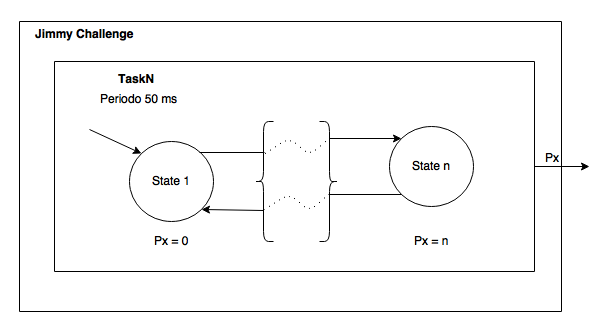
\includegraphics[scale=.60]{img/task_generic.png}
	\caption{Generalizzazione dei task}
\end{figure}

Task:
\begin{itemize}
	\item SonarTask
	\item ButtonTask
	\item BuzzerTask
	\item LedTask
	\item LedPwmTask
	\item LedRgbTask
\end{itemize}
\appendix
\chapter{Elenco dei componenti utilizzati}

\section{Componenti hardware}
\begin{itemize}
	\item Componenti lato client:
	\begin{itemize}
		\item Arduino UNO;
		\item resistori;
		\item sensore di prossimità ad ultrasuoni HC-SR04;
		\item buzzer;
		\item potenziometro;
		\item multiplexer CD4067B;
		\item button;
		\item LED verde;
		\item LED RGB;
		\item LED rosso a 12 pin;
		\item LED giallo a 12 pin;
		\item breadboard;
		\item cavi di collegamento;
	\end{itemize}
\end{itemize}

\begin{itemize}
	\item Componenti lato server:
	\begin{itemize}
		\item Odroid C2;
		\item monitor LCD;
		\item potenziometro;
		\item breadboard;
		\item cavi di collegamento.
	\end{itemize}
\end{itemize}

\section{Componenti software}
\subsection{Librerie Arduino}
\begin{itemize}
	\item \href{http://playground.arduino.cc/Code/NewPing}{NewPing};
	\item \href{https://github.com/bblanchon/ArduinoJson}{ArduinoJson}.
\end{itemize}

\subsubsection{\underline{\href{http://playground.arduino.cc/Code/NewPing}{NewPing}}}\label{sec:newping}
\textbf{Caratteristiche}
\begin{itemize}
	\item Funziona con diversi modelli di sensori ad ultrasuoni: SR04, SRF05, SRF06, DYP-ME007 e Parallax Ping™;
	\item Non ha un \textbf{lag} di un secondo se non si riceve un ping di eco
	\item Ping coerente e affidabile fino a 30 volte al secondo.
	\item Timer interrupt method per sketch event-driven
	\item Metodo di filtro digitale Built-in \texttt{ping\_median()} per facilitare la correzione degli errori.
	\item Utilizzo dei registri delle porte durante l'accesso ai pin per avere un'esecuzione più veloce e dimensioni del codice ridotte.
	\item Consente l'impostazione di una massima distanza di lettura del ping "in chiaro".
	\item Facilita l'utilizzo di più sensori.
	\item Calcolo distanza preciso, in centimetri, pollici e uS.
	\item Non fa uso di \texttt{pulseIn}, in quanto lento e con alcuni modelli di sensore a ultrasuoni restituisce risultati errati.
	\item Attualmente in sviluppo, con caratteristiche che vengono aggiunte e bug/issues affrontati.
\end{itemize}

\subsubsection{\underline{\href{https://github.com/bblanchon/ArduinoJson}{ArduinoJson}}}\label{sec:arduinojason}
\textbf{Caratteristiche}
\begin{itemize}
	\item codifica/decodifica JSON;
	\item API di facile utilizzo;
	\item allocazione di memoria fissa (senza malloc);
	\item nessuna \textit{data duplication} (evitando la copia);
	\item portatile (scritto in C++98);
	\item non ha dipendenze esterne;
	\item libreria leggera;
	\item MIT License.
\end{itemize}

\subsection{IDE utilizzati}
\begin{itemize}
	\item \href{https://atom.io/}{Atom} con \href{ http://platformio.org/}{PlatformIO};
	\item \href{https://www.arduino.cc/en/Main/Software}{Arduino IDE} (per alcuni test sulla comunicazione seriale).
\end{itemize}

\subsection{Linguaggi di sviluppo}
\begin{itemize}
	\item Wiring/C++;
	\item Python;
	\item JSON;
	\item HTML;
	\item ....
\end{itemize}

\subsection{Altro}
\begin{itemize}
	\item \href{http://fritzing.org}{Fritzing} per riportare gli schemi di collegamento.
\end{itemize}
\chapter{Schema di collegamento}
\section{Sketch Arduino - lato client}
\begin{figure}[!ht]
	\centering
	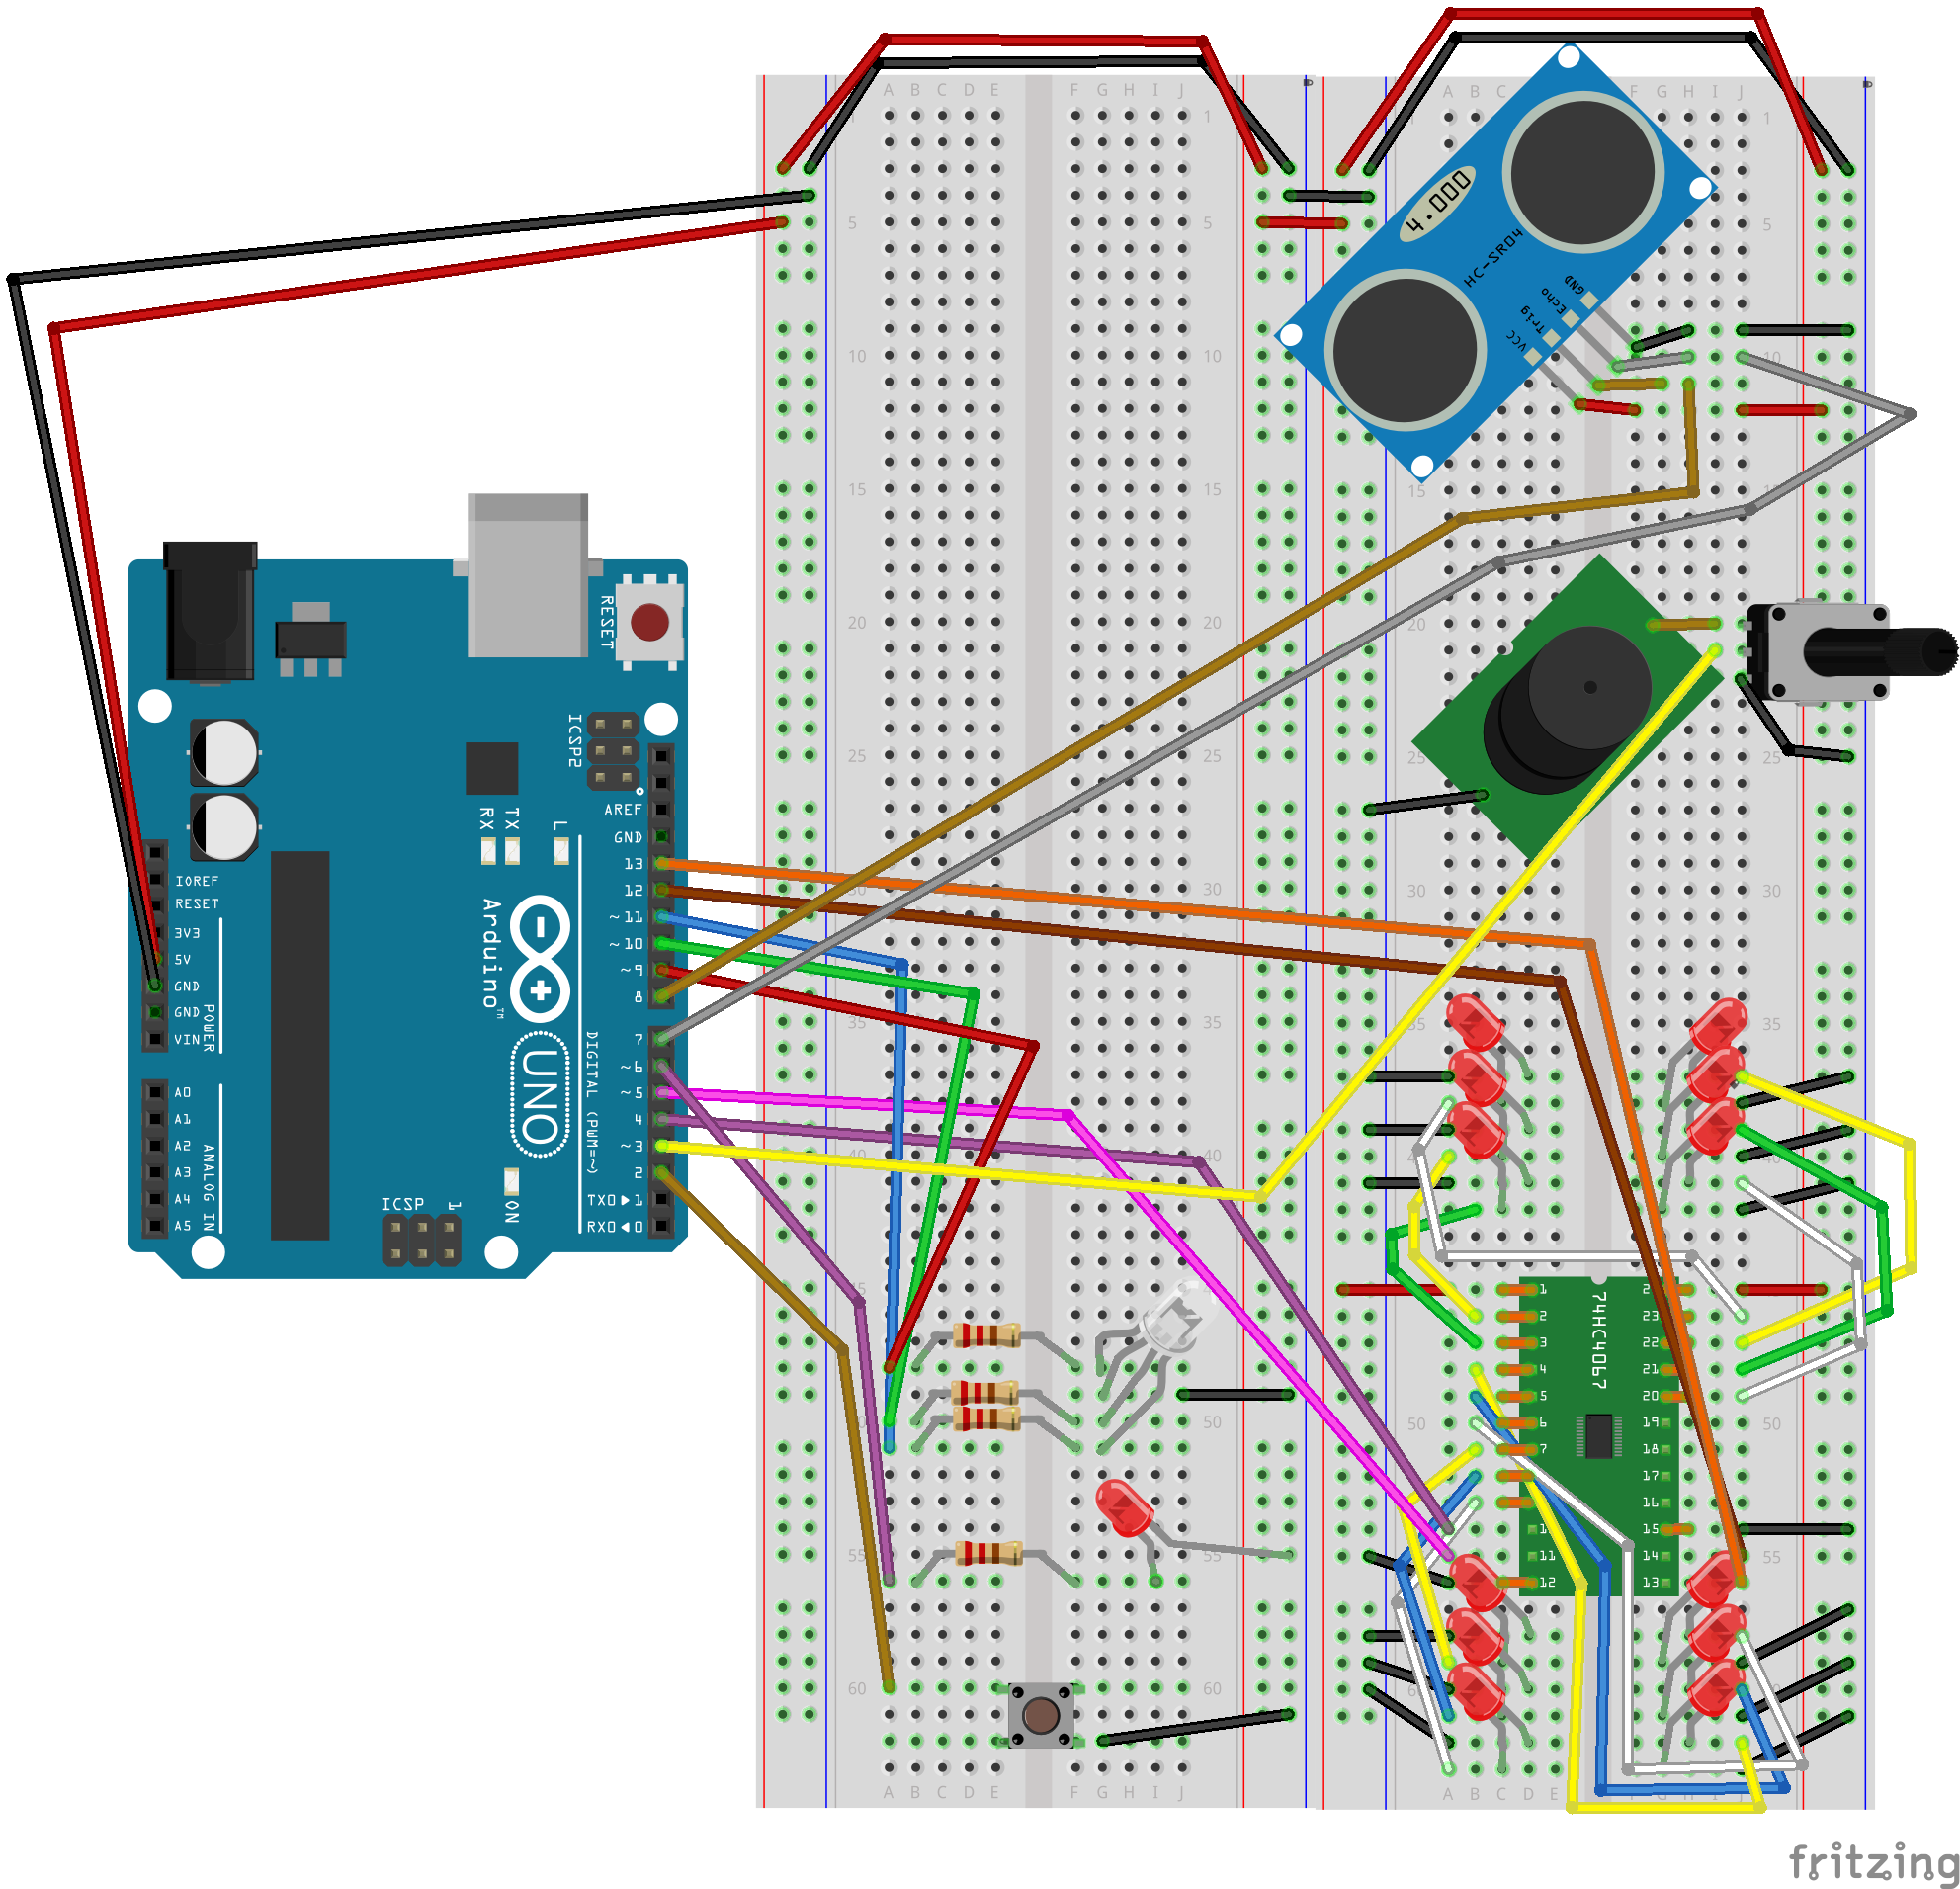
\includegraphics[scale=.60]{img/SketchClient.png}
	\caption{Sketch Arduino - fritzing}
\end{figure}

\begin{figure}[!ht]
	\centering
	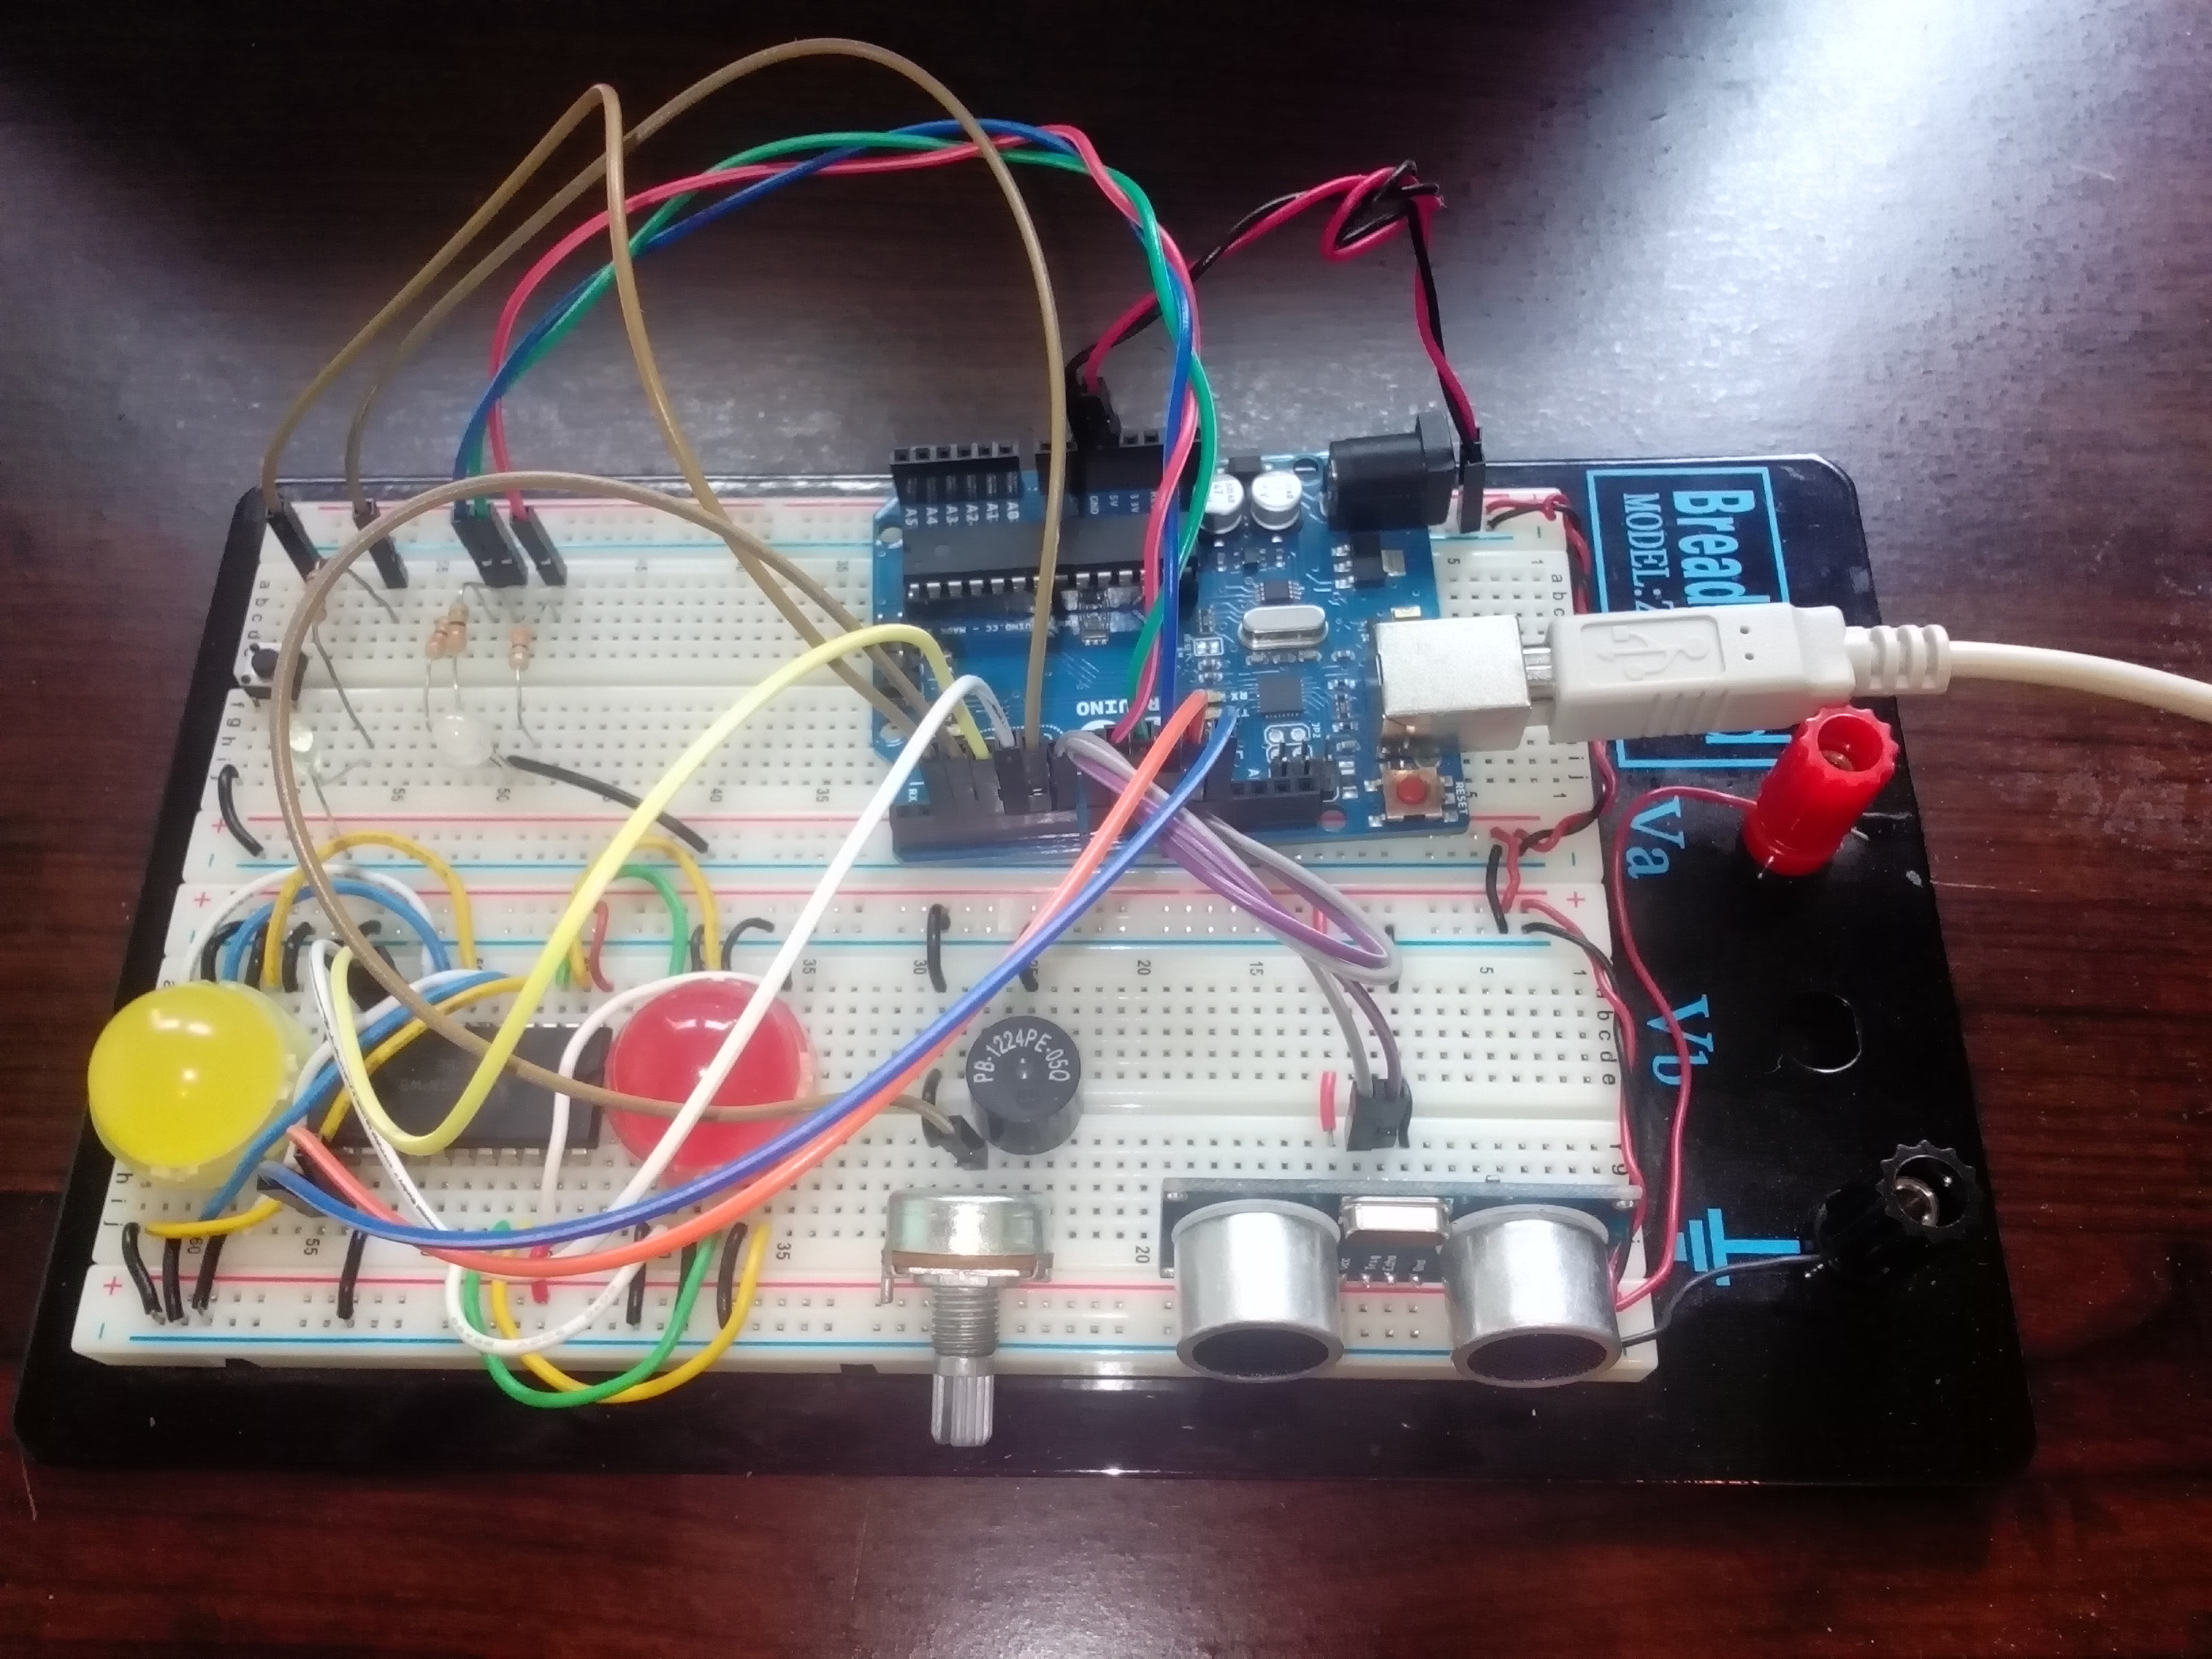
\includegraphics[scale=.08]{img/real1.jpg}
	\caption{Sketch Arduino - realizzazione reale}
	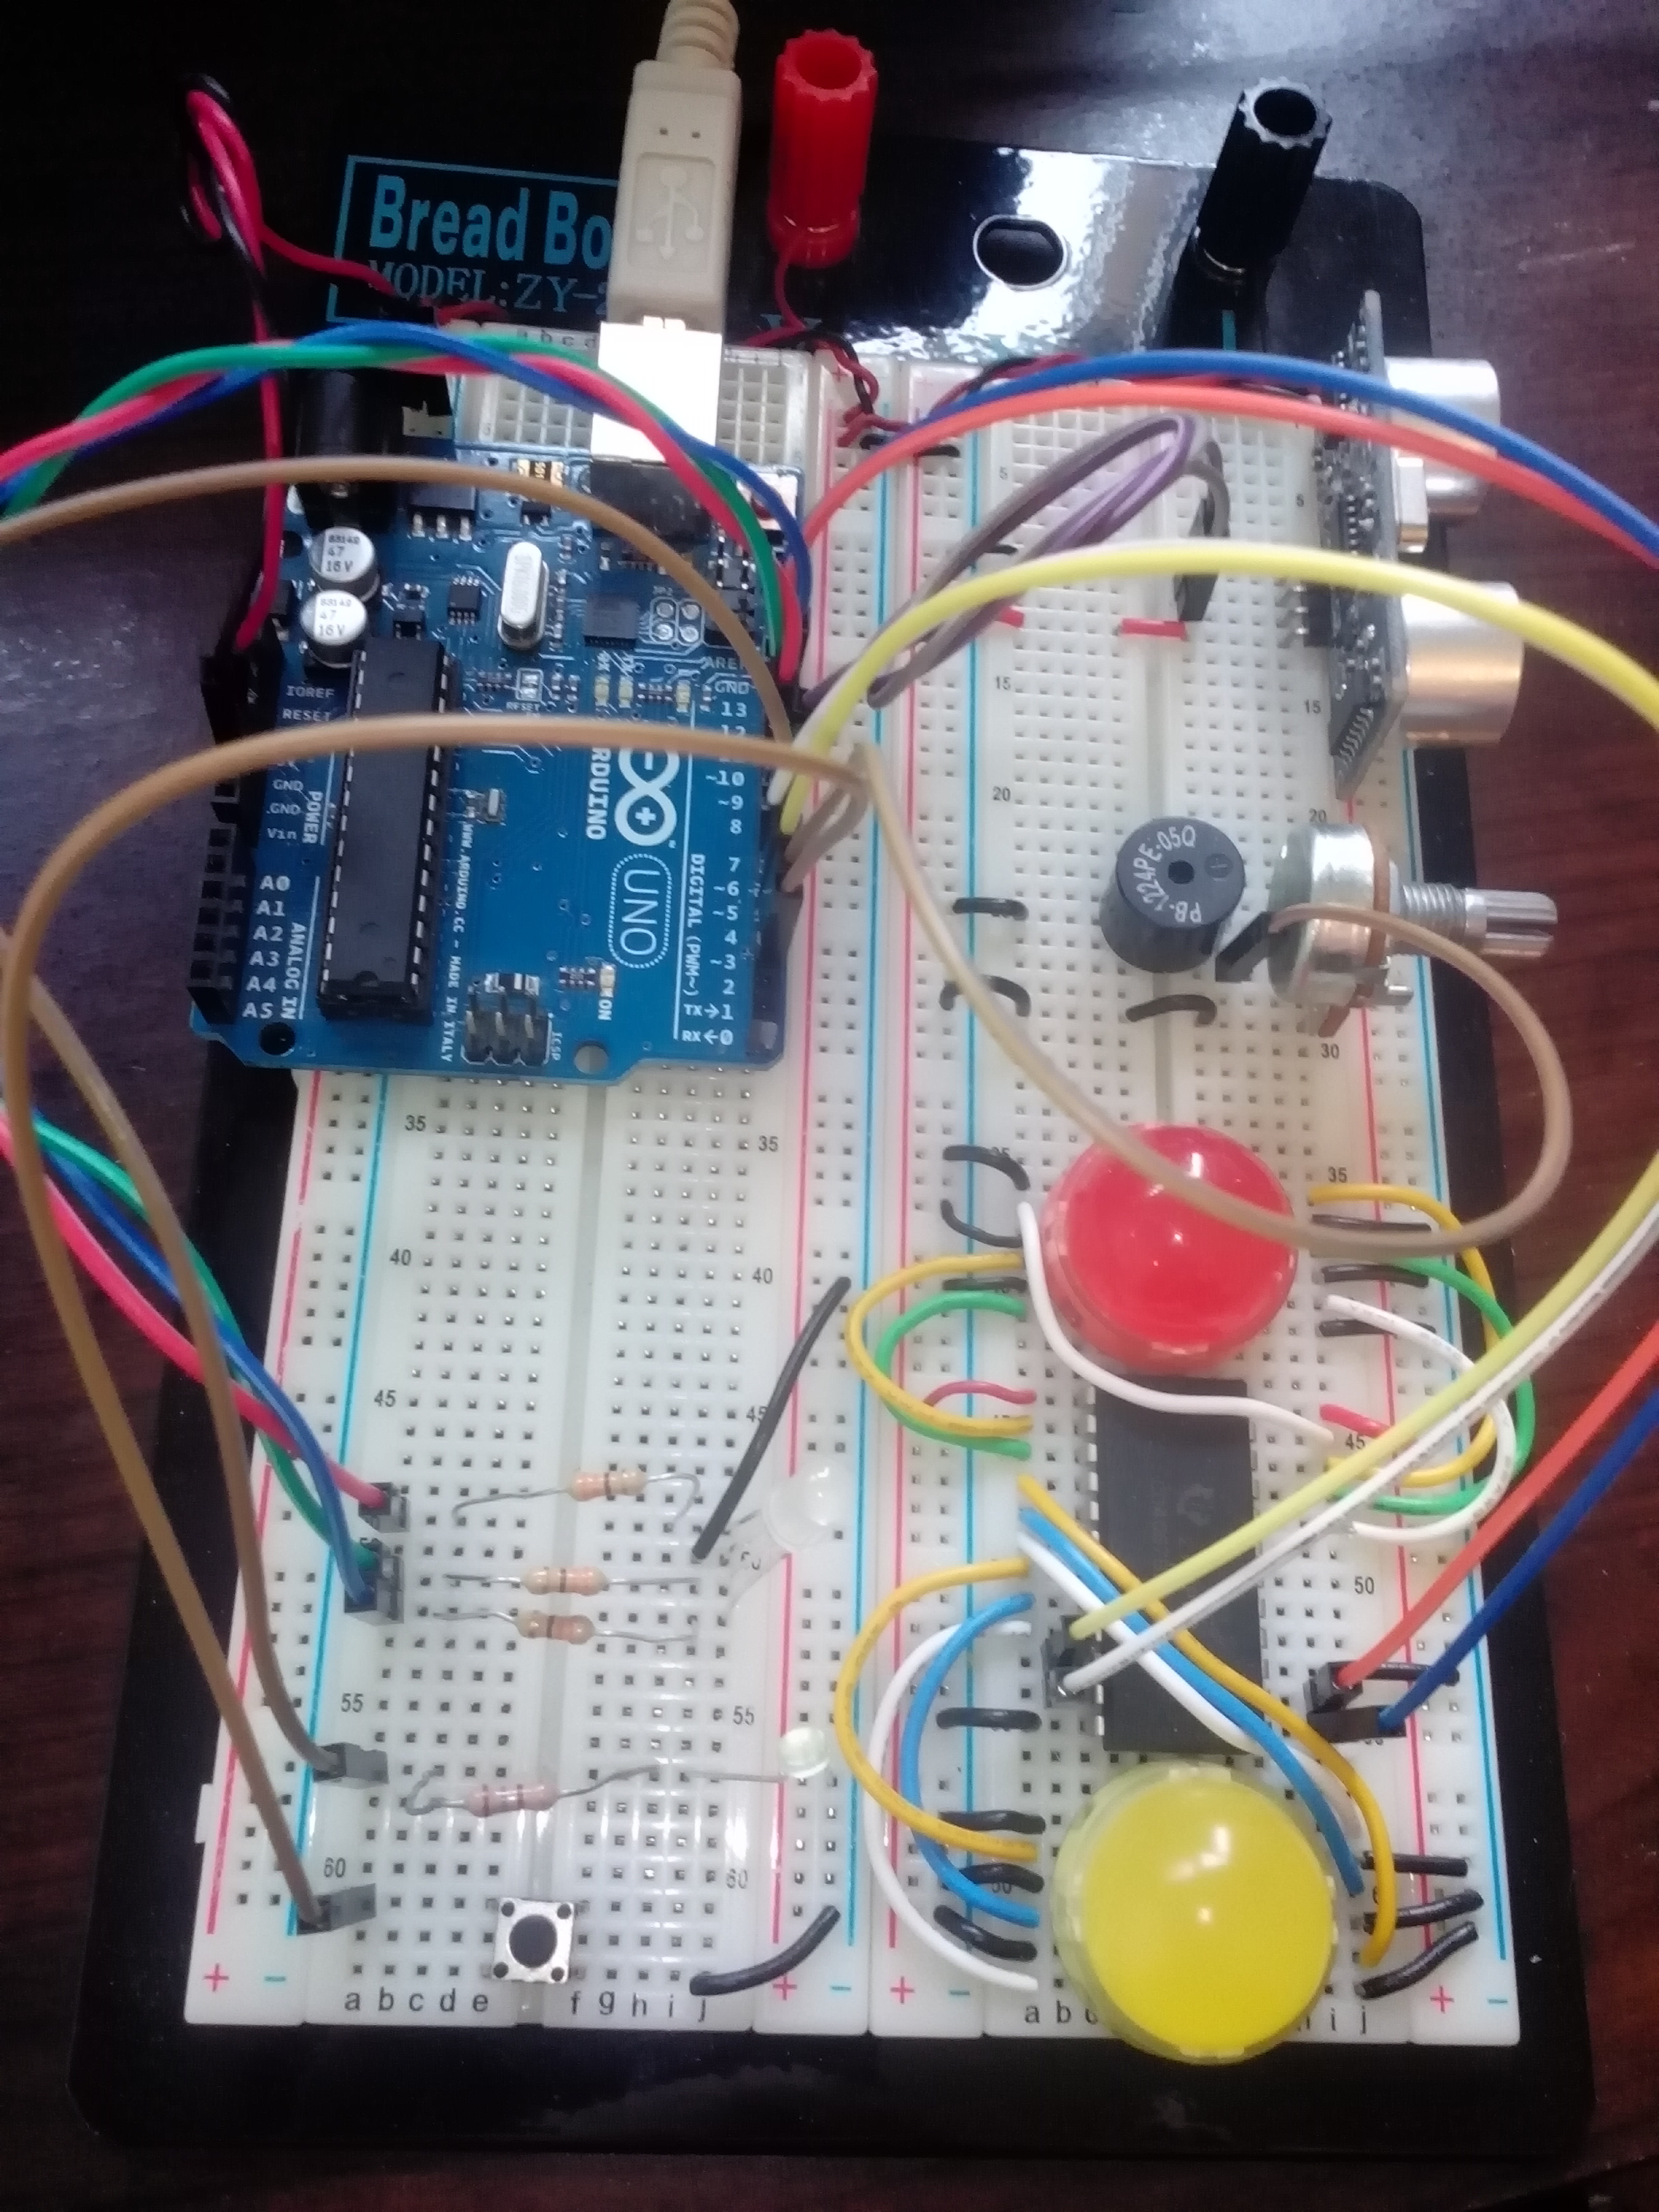
\includegraphics[scale=.08]{img/real2.jpg}
	\caption{Sketch Arduino - realizzazione reale}
\end{figure}

\clearpage
\section{Sketch Odroid - lato server}
\begin{figure}[!ht]
	\centering
	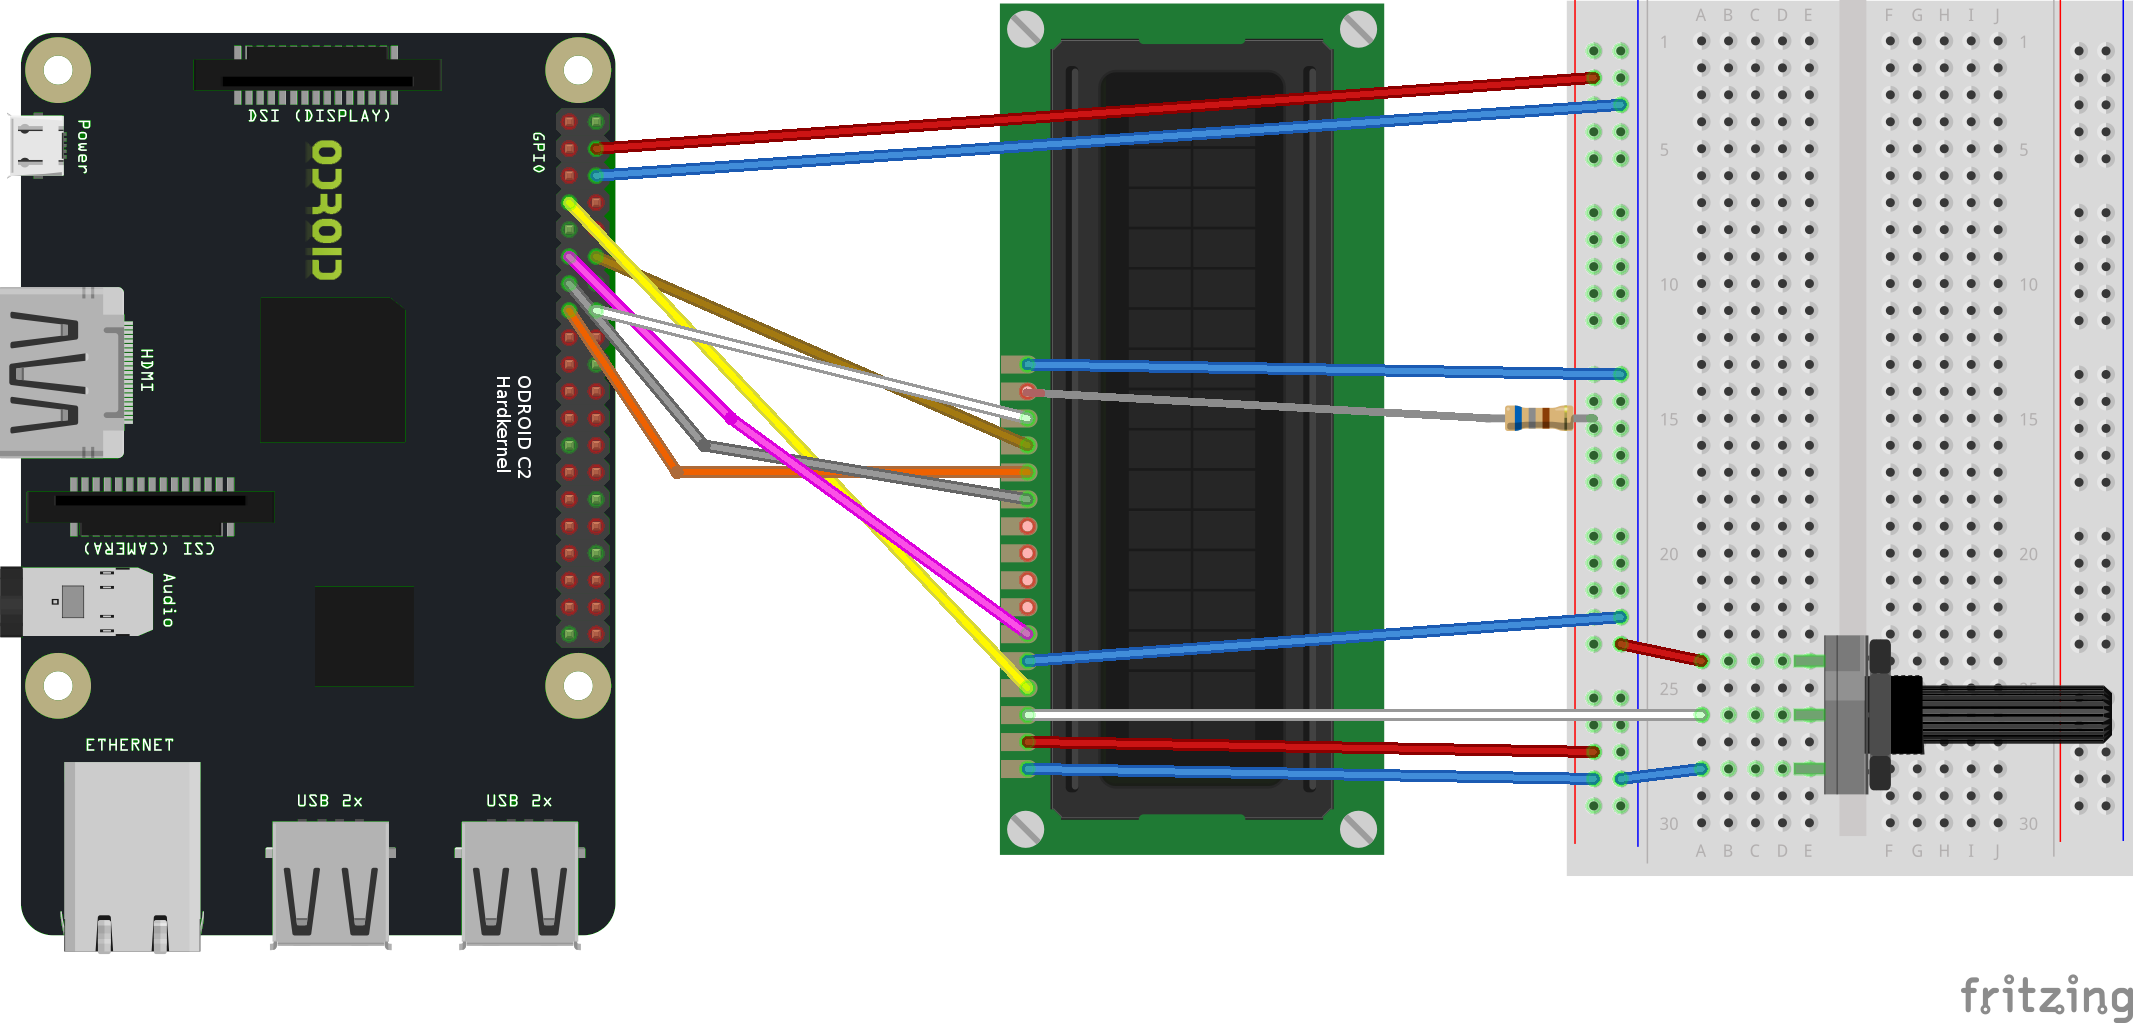
\includegraphics[scale=.2]{img/SketchServer.png}
	\caption{Sketch Arduino - fritzing}
\end{figure}

\begin{figure}[!ht]
	\centering
	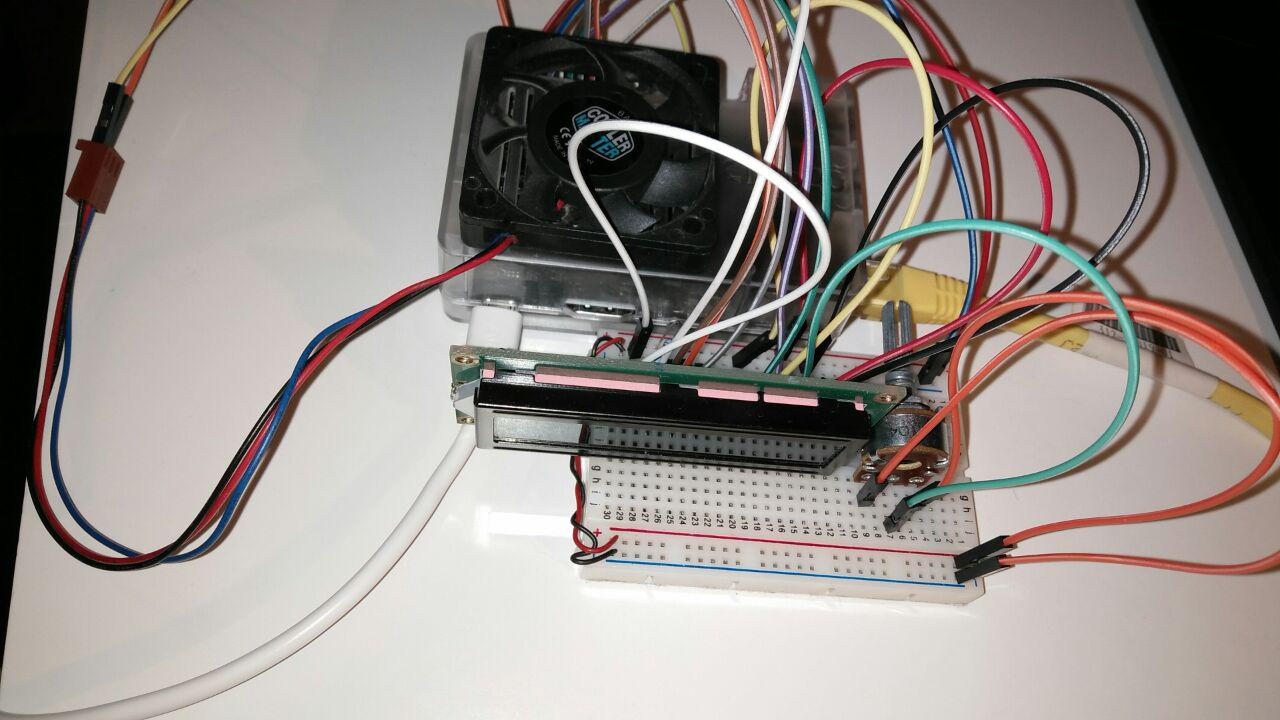
\includegraphics[scale=.3]{img/real3.jpg}
	\caption{Sketch Odroid - realizzazione reale}
	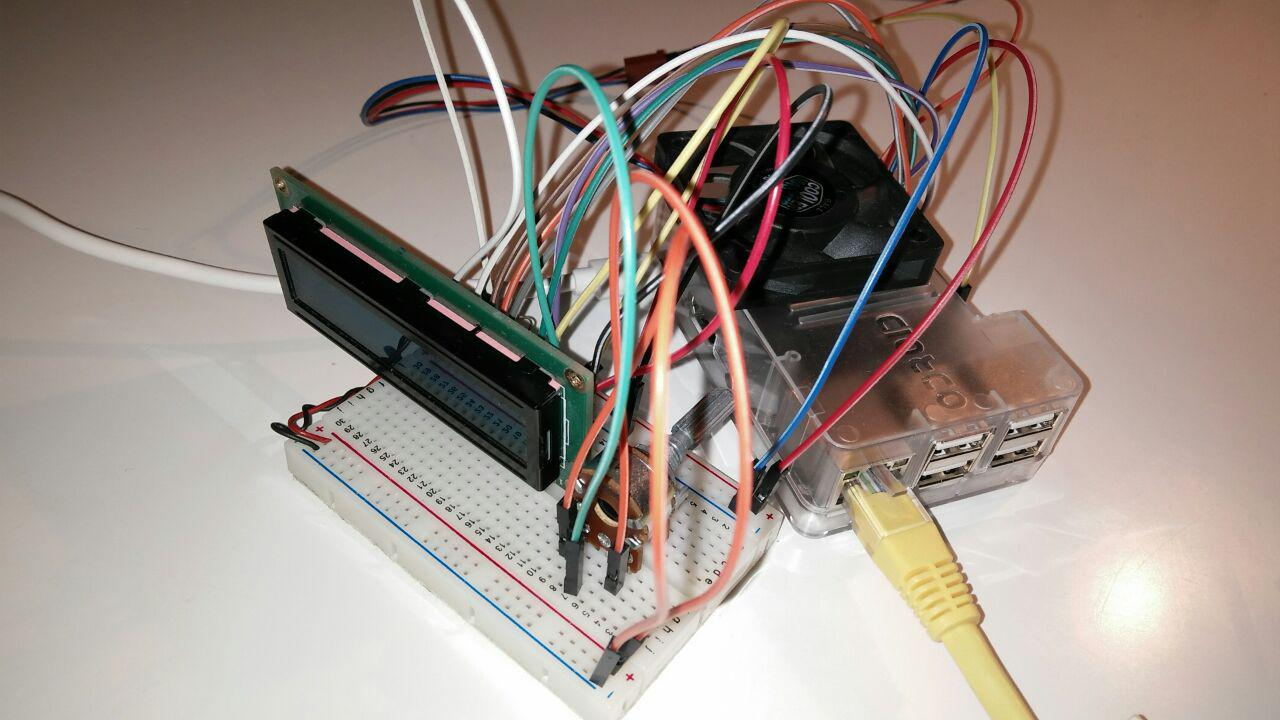
\includegraphics[scale=.3]{img/real4.jpg}
	\caption{Sketch Odroid - realizzazione reale}
\end{figure}
\end{document}               % End of document.
